\chapter{Analysis}

In this chapter we analyze the algorithm used to process EBSD data and explain how to implement it effectively for GPUs. We use the CUDA platform, which is currently the most popular technology for general purpose computing on graphics cards.

\todo{CUDA summary?}

The input for the algorithm consists of one reference and many deformed backscatter patterns which are captured in greyscale images. There may be up to tens of thousands of them. In general, the format of the pictures is not important, as long as it is possible to load them from disk quickly. For example, our testing data consists of 15000 images saved in TIFF format without any compression. Each picture has resolution of approximately $900 \times 900$ pixels and each pixel is represented by a 16 bit unsigned integer --- the higher the integer, the higher is the luminosity of the pixel.

The result of the algorithm is a list of two--dimensional vectors that we write to the standard output.

From a high--level point of view, the algorithm first loads reference pattern from disk. Then it goes through a list of file names of deformed images and does 3 steps with each:
\begin{enumerate}
	\item Load a deformed pattern from disk.
	\item Compare the deformed and reference patterns.
	\item Write the resulting offsets to standard output.
\end{enumerate}
While the steps 1 and 3 have to be done by the CPU, the second step is suitable for execution on a GPU.

As explained in previous chapter, the comparison of two patterns is done by cross--correlating several subregions of the images and then finding the offset for which the correlation is maximal. Location, size and number of the subregions is a parameter for the algorithm, but we expect that there will be tens of subregions with size in the order of $100 \times 100$ pixels. All the subregions in all the images are processed independently from each other, providing a great opportunity to utilize data parallelism.

The processing of each subregion is done in several steps:
\begin{enumerate}
	\item Normalize the pixels of the subregion --- compute its mean and subtract it from each pixel
	\item Cross--correlate deformed region with the reference one
	\item Find the position of the maximum (argmax) in the cross--correlation
	\item Use the neighborhood of the maximum to ``interpolate'' and find the most probable offset of the subregion with subpixel accuracy
\end{enumerate}
That summarizes the algorithm and in the next section we describe its implementation.


\section{Implementation overview}

\begin{figure}
	\centering
	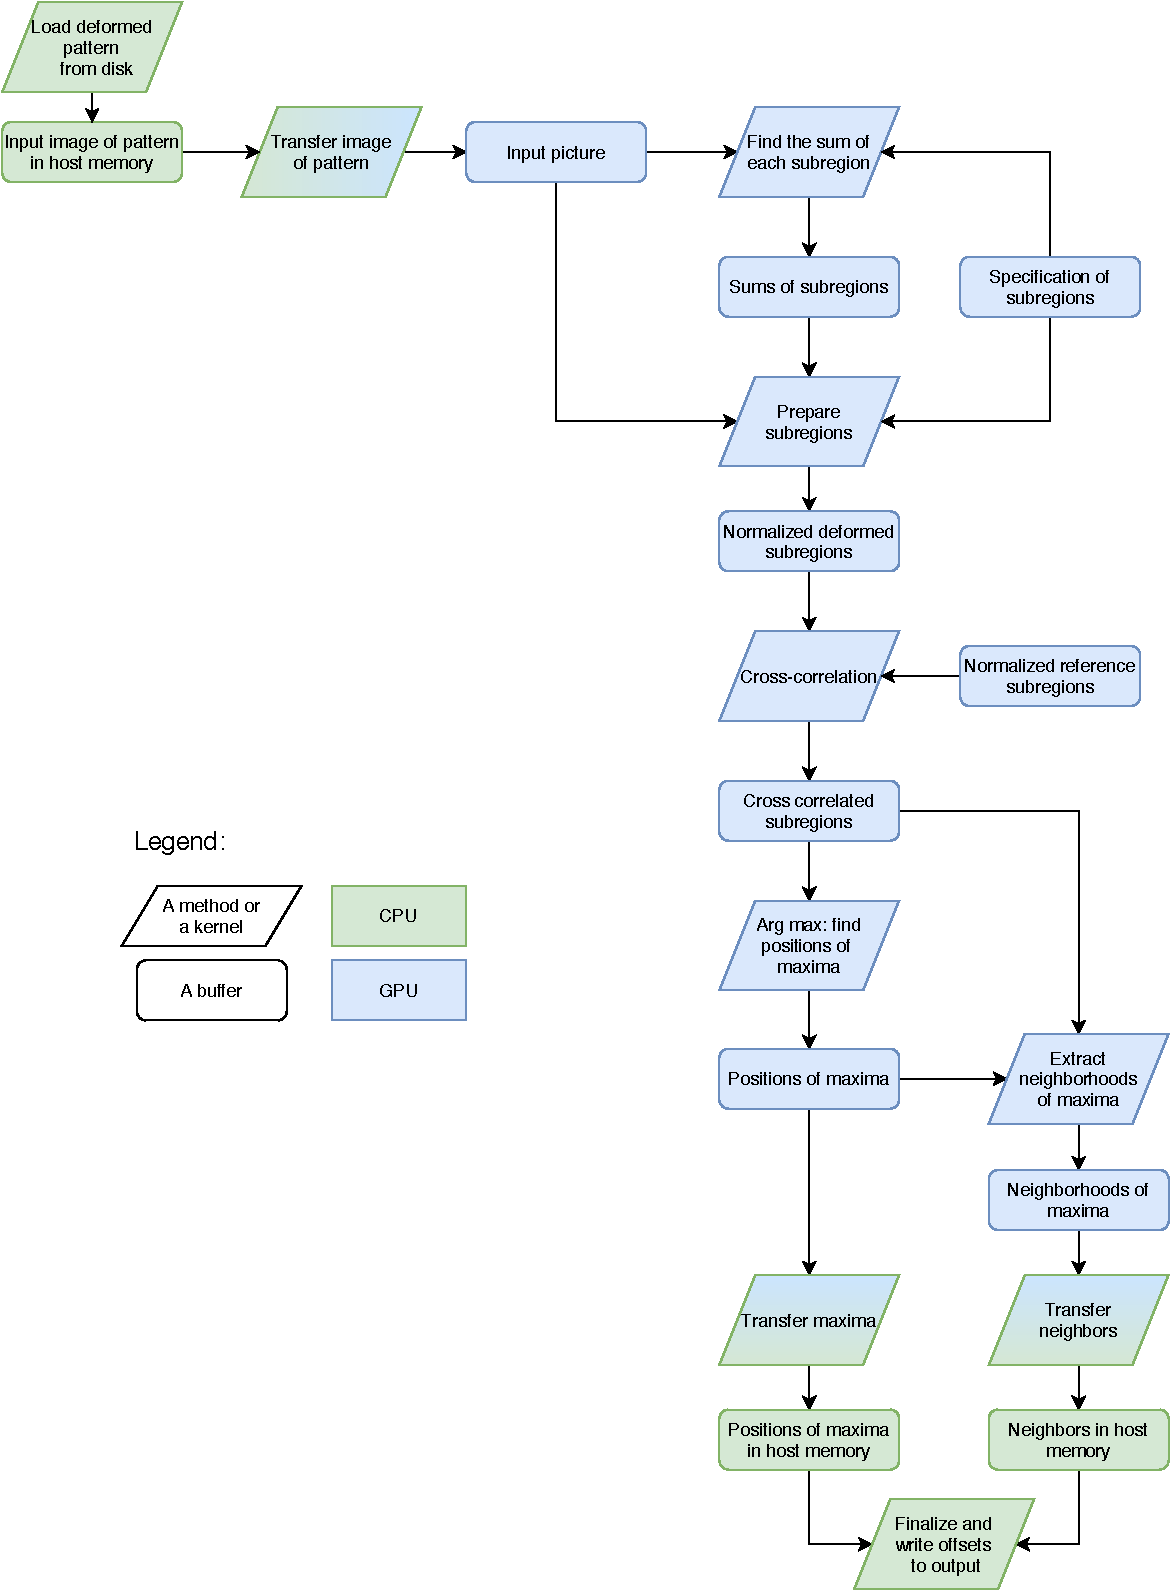
\includegraphics[width=\textwidth]{img/overview}
	\caption{Processing of one deformed pattern.}
	\label{overview}
\end{figure}

\Cref{overview} shows the data flow of the implementation and its decomposition into kernels. The processing starts with loading an image of a pattern from disk and its transfer to GPU. We transfer the whole pattern, as opposed to transferring only the subregions of interest.  Although we may end up copying data that the GPU never uses, this approach turned out to be better, because then we can utilize GPU when slicing the pattern into subregions. Moreover, we expect the regions to overlap in typical use case, so transferring the whole pattern copies less data.

The image is represented as an array of all the pixels in row--major order. Each pixel is an unsigned integer. 

Next, we need to prepare the data for cross--correlation --- slice the image of deformed pattern to subregions and normalize them by subtracting the respective means. It is done in two kernels: the first one computes the sum of pixels of each subregion using parallel reduction. The second kernel extracts the subregions from the pattern, so that they are organized one after another in the output buffer: first, there all the pixels of the first subregion in row--major order, then all the pixels from the second and so on. Moreover, the kernel uses the sums from the first kernel to compute the mean for each region and subtracts it from each pixel of respective subregion.

The following part cross--correlates the normalized deformed subregions with reference ones. Since each deformed pattern is compared to the same reference, we pre-compute it and store it in a buffer on the GPU before loading the first deformed pattern.

Then, we analyze the result of the cross--correlation --- we find where is the maximum of each subregion using parallel reduction. The result is an array of coordinates of the maximum values (we are not interested in the values themselves). The next kernel then extracts a square shaped neighborhood of each maximum into one continuous buffer, so it can be transferred to the CPU memory together with the positions of the maxima.

The last part of the algorithm fits a continuous quadratic function to the neighborhood and then finds its maximum. We did not implement it for GPU, because it is not computationally demanding. It processes only a small neighborhood compared to the expected size of subregions. That also makes it cheap to transfer the maxima and neighborhoods from GPU to finish the computation on CPU and write the results to the output.

The decomposition into kernels is mostly determined by the need of global barriers. Both finding of sum and argmax use parallel reduction, which has to fully finish before any of its results are complete. The kernel that extracts the subregions from the pattern is necessary, to simplify the cross--correlation and allow usage of third party libraries (see \cref{fft}, where the implementation of cross--correlation is explained).

To illustrate the data flow better and reason about it, \cref{params} summarizes parameters of the algorithm and \cref{buftypes} shows all buffers used on GPU with their sizes. The kernels that compute sums and normalize the subregions both work with $W_r \cdot H_r \cdot S$ items (i.e. all subregions). The cross--correlation has nearly four times as big output, which is then processed by the arg max kernel. After the maximum reduction, the buffers that are transferred to the CPU memory are quite small.

% Please add the following required packages to your document preamble:
% \usepackage{booktabs}
\begin{table}[]
	\centering
	\begin{tabular}{@{}llr@{}}
		\toprule
		Parameter                  & Label            &    Typical value \\ \midrule
		Size of input pattern      & $W_p \times H_h$ & $900 \times 900$ \\
		Number of subregions       & $S$              &               50 \\
		Size of a subregion        & $W_r \times H_r$ & $100 \times 100$ \\
		Diameter of a neighborhood & $F$              &                5 \\ \bottomrule
	\end{tabular}
	\caption{Summary of algorithm parameters with example values that show their order of magnitude.}
	\label{params}
\end{table}

\begin{table}[]
	\begin{tabular}{@{}lll@{}}
		\toprule
		Buffer                          & Type         & Number of elements             \\ \midrule
		Input picture                   & uint16       & $W_p \cdot H_p$                \\
		Sums of subregions              & uint32       & $S$                            \\
		Specification of subregions     & uint32 pair  & $S$                            \\
		Normalized deformed subregions  & float/double & $W_r \cdot H_r \cdot S$        \\
		Normalized reference subregions & float/double & $W_r \cdot H_r \cdot S$        \\
		Cross--correlated subregions    & float/double & $(2W_r-1)\cdot(2H_r-1)\cdot S$ \\
		Positions of maxima             & uint32 pair  & $S$                            \\
		Neighborhoods of maxima         & float/double & $F^2 \cdot S $                 \\ \bottomrule
	\end{tabular}
	\caption{Summary of GPU buffers with their data types and size.}
	\label{buftypes}
\end{table}

buffer data types

\subsection{Task parallelization}

Since some parts of the algorithm are done on CPU and some on GPU (see color distinction in \cref{overview}), it is possible to parallelize them. There are 3 parts separated by data transfer between the main and the GPU memory: CPU first loads a pattern, GPU processes it, and then CPU does the finalization of results. It is desirable that we parallelize those tasks, so that GPU is fully utilized and never waits for the CPU.

\begin{figure}
	\centering
	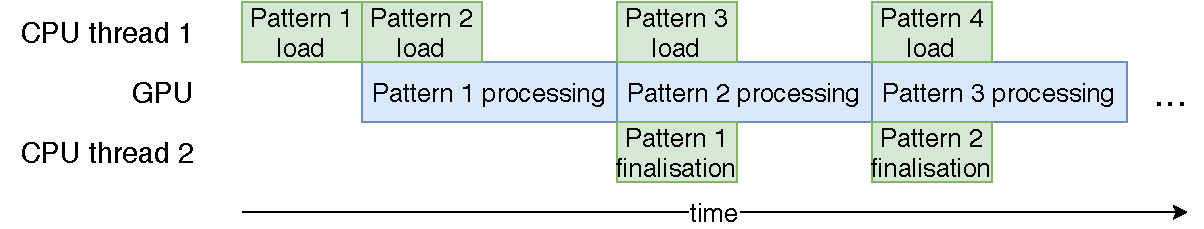
\includegraphics[width=\textwidth]{img/CPUGPUparal}
	\caption{Parallelization of GPU and CPU work.}
	\label{pipeline}
\end{figure}

\Cref{pipeline} shows how the work can be can be parallelized using a pipeline-based design. We use 2 additional CPU threads. While the GPU processes $i$-th pattern, one CPU thread already loads pattern $i+1$ and the second thread finalizes pattern $i-1$. The CPU work still takes much less time, so it is enough to start the load of pattern $i$ once processing of pattern $i-2$ finishes (and processing $i-1$ starts). That way, we do not need queues to pass work, we just need 2 buffers: one for writing the processed/prepared data and one for reading data to process. In the next iteration, we just swap the buffers.

We also partially take advantage of the fact that GPUs are able to run a kernel, copy data from and to memory at the same time. Actually, all transfers run in parallel with kernel execution. The host--device copy of input takes place right after the CPU loads the pattern from disk. Similarly, once the maxima and neighborhoods are prepared on the GPU, we start asynchronous transfer of the results and GPU starts computing the next pattern immediately. Unfortunately, this optimization does not affect performance much, since the copying between GPU and CPU memory takes only a small fraction of overall time.

In the following sections, we describe the implementation details of each individual kernel.




\section{Sum computation}

Computation of sum is a textbook example of parallel reduction. \cite{parallelReduction} explains how to implement it on modern GPUs. Since it is very expensive to communicate between arbitrary threads during computation, the reduction is separated into two steps: first, we reduce the data within each block individually and only then we synchronize single value for each block.

The major difference for our case is that we compute a sum for each subregion, instead of computing a sum for the whole input data. The problem is that we cannot load values of two different subregions into one block. We solve this by assigning whole blocks to the subregions rather than just assigning threads to pixels. Let $B$ and $P$ denote one block size and total number of pixels in one subregion, respectively. Then we use a group of $S_1~=~\ceil{\frac{P}{B}}$ blocks for reduction of each subregion. Inside each block, we assign one thread per pixel in row-major order, so adjacent threads access adjacent data. It also means that the last block in each group is not fully utilized, because there is no more pixels in the subregion.

Once each thread loads its data, it is possible to reduce them fast within each block. We use warp--level shuffle instructions, which allows the threads in one warp to exchange data in registers. \Cref{warp_reduce} shows how it is possible to get sum of values in 8 threads. It can be expanded to size of warp, i.e. 32 threads. To reduce the whole block, we use the warp reduction in two steps. First, we perform the reduction within each warp and save the values into shared memory. Maximum number of threads in one block is 1024 in CUDA and warp size is 32 so we get at most $1024/32 = 32$ values. That means one warp is enough to reduce them into one resulting value.

\begin{figure}
	\centering
	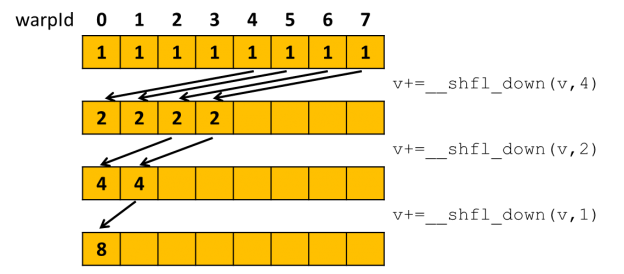
\includegraphics[width=0.7\textwidth]{img/warp_reduce}
	\caption{An example of warp--level reduction for 8 threads \cite{parallelReduction}. \emph{warpId} is a number of thread within its warp.}
	\label{warp_reduce}
\end{figure}

After reduction within each block, we need to update the resulting values in global memory, which requires more blocks working with the same value, possibly in parallel. On modern hardware, we solve such situations with atomic operations --- in our case of computing the sums it is \emph{atomic add}. The solution is feasible for us, since it is safe to assume that not many blocks access the same value. The typical size of one subregion is $100 \times 100$ which is the total of 10000 pixels. If we set the block size to 1024 (there is no reason not to use the maximal possible value --- no register or shared memory pressure), then only 10 blocks compute the sum of one subregion.

It is possible to further optimize the described technique by increasing the number of values each thread loads before the reduction begins. The problem is that half of the threads do (almost) nothing useful in the whole reduction: each of them only loads one value in the very beginning and immediately passes it to another thread which does the actual sum. So instead of loading only one value, each thread loads $N$ values and all the threads are utilized in the first part of the algorithm. It also means that we need $N$ times less blocks which may cause that for too high $N$, there will not be enough blocks to utilize the GPU. We measure the impact of the parameter in section ??.



\section{Cross--correlation}
Cross--correlation is the core of the algorithm implemented in this thesis and it is also the most computationally expensive part. We first describe a naive algorithm designed directly from the definition. Then we explain another implementation that uses discrete Fourier transform. The reason why we implement two versions is that although the Fourier transform based implementation has better asymptotic complexity, the subregions may not be big enough to reflect it.

The input for cross--correlation are two images, in our case it is a deformed and a reference subregion. More precisely, there are several pairs of subregions, but since they are completely independent, we explain the algorithm for one pair only. With respect to the definition in \cref{cross-corr-def}, we cross--correlate the reference with deformed subregion, i.e. $reference \star deformed$, not the other way around. Also, both subregions are of the same size, which simplifies some aspects of the algorithm.

A serial algorithm for cross--correlation is shown in algorithm \ref{crossAlgo}. It is directly based on the definition. It iterates over all possible shifts between the images (subregions), i.e. $\forall [shiftX, shiftY] \in (-W_s, W_s) \times (-H_s, H_s)$. Shifts that are further from zero than width (height) of the picture are always zero, since the second subregion is shifted so far that they do not overlap at all. For each of the shifts $[shiftX, shiftY]$, we sum over the products of pixels that overlap when we shift the deformed subregion by shiftX pixels horizontally and by shiftY vertically.



\begin{algorithm}
	\caption{Serial algorithm that computes cross--correlation.}
	\label{crossAlgo}
	\KwIn{reference: an array of pixels of a reference subregion \newline
		  deformed: an array of pixels of a deformed subregion \newline
	      $W_s, H_s$: size of both subregions}
	\KwOut{result: cross--correlation between reference and deformed subregions}
	\vspace{5px}
	
	\For{$\text{shiftX} \in (-W_s, W_s)$}{
		\For{$\text{shiftY} \in (-H_s, H_s)$}{
			sum = 0\;
			\For{$x \in [0, W_s)$}{
				\For{$y \in [0, H_s)$}{
					shiftedX = x + shiftX\;
					shiftedY = y + shiftY\;
					\If{$\text{shiftedX} \in [0,W_s]$ \textbf{and} $\text{shiftedY} \in [0,H_s]$}{
						sum += reference[x,y] * \newline deformed[shiftedX, shiftedY]\;
					}
				}
			}
			result[shiftX, shiftY] = sum\;
		}
	}
\end{algorithm}

\begin{algorithm}
	\caption{Pseudocode of CUDA kernel that computes cross--correlation.}
	\label{crossKernel}
	
	shiftX = threadId.x\;
	shiftY = threadId.y\;
	intervalX = $\text{shiftX} < 0$ ? $[-\text{shiftX}, W_s]$ : $[0, W_s - \text{shiftX}]$\;
	intervalY = $\text{shiftY} < 0$ ? $[-\text{shiftY}, H_s]$ : $[0, H_s - \text{shiftY}]$\;
		
	sum = 0\;
	\For{$x \in [0, \text{intervalX})$}{
		\For{$y \in [0, \text{intervalY})$}{
			shiftedX = x + shiftX\;
			shiftedY = y + shiftY\;
			sum += reference[x,y] * deformed[shiftedX, shiftedY]\;
		}
	}
	result[shiftX, shiftY] = sum\;

\end{algorithm}

The inner two loops of the algorithm iterate through all pixels of the reference image. However that is not necessary for all shifts, since for most of them only smaller parts of the images overlap (the only shift that requires iteration through all points is $[0,0]$). The if statement then filters out the pixels that do not overlap for specific shift. For performance reasons, we can get rid of the if statement, if we rewrite the two inner loops to always stay within the boundaries of the images.

We will reason only about $shiftX$, since the same argumentation applies to $shiftY$. So we are asking the following question: for which $x \in [0, W_s)$, it holds that $(x + shiftX) \in [0, W_s)$, if $shiftX \in (-W_s, W_s)$? We divide $shiftX$ into negative and nonnegative values:
\begin{itemize}
	\item $\forall shiftX \in (-W_s, 0): (x + shiftX) \in [0, W_s) \iff x \in [-shiftX, W_s]$
	\item $\forall shiftX \in [0, W_s): (x + shiftX) \in [0, W_s) \iff x \in [0, W_s - shiftX]$
\end{itemize}
This gives us an interval through which we iterate $x$ in the inner loops for each \IT{shiftX}. Similar modification applies for the y loop based on \IT{shiftY} as well.

The modified algorithm written as a CUDA kernel is listed in algorithm~\ref{crossKernel}. We implemented the algorithm for CUDA by parallelizing over the outer two loops. That means each thread computes one shift and thus one value of the result. It uses two--dimensional blocks, so we can just use the two indices as \IT{shiftX} and \IT{shiftY}. For computing more subregions at a time, we simply use more threads.

The described algorithm has asymptotic time complexity $\mathcal{O}(W_s^2H_s^2)$. In the following section, we describe a way to compute two--dimensional cross--correlation in $\mathcal{O}(W_sH_s\log_2(W_sH_s))$ using Fourier transform.

\subsection{Discrete Fourier transform}
\label{fft}

We first define \emph{circular cross--correlation}, which is a way to cross--correlate periodic functions. Then, we define \emph{discrete Fourier transform} and show how it is used to compute circular cross-correlation. Finally we show how to get the cross--correlation we need in the implementation. All is described for one--dimensional case only, since two--dimensional would be analogous.

Let $N \in \mathbb{N}$, $\{x_n\} = x_0, x_1, \dots , x_{N-1}$ and $\{y_n\} = y_0, y_1, \dots , y_{N-1}$ be series of complex numbers. Then their circular cross--correlation is another series of $N$ numbers defined by the formula
\[
\{\mathbf{x} \star \mathbf{y}\}_n = \sum_{l=0}^{N-1}x^\star_ly_{(n+l)\bmod N}
\]

%We can see that the definition is very similar to cross--correlation of two functions (see \cref{cross-corr-def}), except here we do.

Circular cross--correlation can be interpreted as a cross--correlation of two periodic functions. For any periodic function with period $N$, we only need $N$ consecutive values to represent, since the rest of the function repeats the same values. At the same time, given two periodic discrete functions $f, g : \mathbb{Z} \rightarrow \mathbb{C}$ with period $N$, their cross--correlation $f \star g$ is also periodic with the same period. So if we interpret the series in the definition of circular cross--correlation of as periodic functions, then the resulting series represents (non-circular) cross--correlation of the functions.

%The $\mod$ operation causes that whenever the $n+l$ is greater or equal than $N$, we ``circulate'' and take 

The circular cross--correlation can be quickly computed by using the discrete Fourier transform.

The discrete \emph{Fourier transform} is a function $\mathcal{F}: \mathbb{C}^N \times \mathbb{C}^N$ that transforms a series of $N \in \mathbb{N}$ complex numbers $\{x_n\} = x_0, x_1, \dots , x_{N-1}$ into another $N$ complex numbers $\{X_n\} = X_0, X_1, \dots , X_{N-1}$, which are defined as follows:
\[
X_k = \sum_{n=0}^{N-1} x_n \cdot e^{-\frac{i2\pi}{N}kn}.
\]
The Fourier transform is invertible, so if $\mathcal{F}(\mathbf{x}) = \mathbf{X}$, then $\mathcal{F}^{-1}(\mathbf{X}) = \mathbf{x}$.

Fourier transform has a broad range of practical applications --- it is used for example in digital signal processing, solving partial differential equations or big numbers multiplication. It can be used to quickly compute the circular cross--correlation using the following theorem \cite{proakis2004digital}.

Let $N \in \mathbb{N}$, $\{x_n\} = x_0, x_1, \dots , x_{N-1}$, $\{y_n\} = y_0, y_1, \dots , y_{N-1}$ be series of complex numbers and let $\{X_n\}$, $\{Y_n\}$ be their Fourier transforms. Then, we can compute \emph{circular cross--correlation} like so: 
\[
\mathcal{F}^{-1}\{X^\star \cdot Y\}_n = \sum_{l=0}^{N-1}x^\star_ly_{(n+l)\bmod N},
\]
where $\cdot^\star$ denotes the complex conjugate and $\cdot$ denotes element by element multiplication.

In other words, in order to compute circular cross--correlation of two series $\{x_n\}$ and $\{y_n\}$, we first compute their Fourier transforms $\{X_n\}$ and $\{Y_n\}$, then multiply corresponding elements of the transformed series and finally we do an inverse Fourier transform. We do all of this, because we are able to compute both the discrete Fourier transform and its inverse in time $\mathcal{O}(N \log N)$, which gives us the overall asymptotic time $\mathcal{O}(N \log N)$ compared to $\mathcal{O}(N^2)$ when computing the circular cross--correlation from definition.



\section{Arg max}


\section{Least squares implementation}